\section{Realistic Models of Recommendation Graphs}
%We realize that the models described previously are a bit
%theoretical.
Even though we studied the fixed-degree model in detail, recommendation systems based on relevance in practice
will not have edges that are spread uniformly at random. Items that are
about specific topics are much more likely to interlink within
themselves than to those outside that topic, leading to
clusters of recommendations.

To understand this substructure in underlying
graphs in practice, we compiled results from several e-commerce retailers that
have been aggregated and anonymized in the table shown below. For each
retailer, we compiled the product ontology present within the
site that places a product in this tree-like categorization. E.g., a
juicer called ``Breville Juice Fountain Plus'' is in the tree path:
Home $\rightarrow$ Juicers $\rightarrow$ High Speed Juicers
$\rightarrow$ Breville Juice Fountain Plus. We then examined the
recommendations from products at different depths of the hierarchy. In
the table in Figure~\ref{fig:hier} we examined the edges adjacent to
products at depth 4 or greater. We calculated the percentage of edges
connecting to products that had different least common ancestors (LCA) with the current product.  We
then randomized the edges so that we can compare how the graph would
have looked if there was no substructure and re-calculated the
distribution of the edges and the LCA levels. We noticed that the
uniform distribution had edges that had very shallow LCA indicating that
most edges did not follow the product hierarchy while in reality,
the endpoints of edges recommended had much deeper LCA meaning recommendation edges were clustered based on the product hierarchy. This led us
to formalize this new model of input graphs that we study in Subsection~\ref{hierarchy}
as the {\em hierarchical tree model}.

\begin{figure}[h]
  \centering
  \begin{tabular}{ |c|c|c|c|c|c|c|c|c|c| }
    \hline
    $LCA Level$ & 0 & 1 & 2 & 3 & 4 & 5 & 6 & 7 \\ \hline
    Uniform & 13.4 & 69.7 & 12.5 & 2.6 & 1.2 & 0.6 & 0.0 & 0.0 \\ \hline
    Hierarchical & 7.1 & 1.9 & 8.0 & 24.9 & 52.3 & 5.5 & 0.2 & 0.1\\
    \hline
  \end{tabular}
  \caption{Percent edges for depth-4 products by LCA of endpoints in reality (from hierarchical data) and simulated Uniform.}\label{fig:hier}
\end{figure}

In a second analysis, we simply truncated the product hierarchy
at depth 3 and collected the resulting disjoint clusters in the hierarchy. We
then examined all the recommendations and partitioned them into those going between each pair of these clusters. In a uniform distribution, we would expect the
edges to be equally likely to span across each pair of clusters
(assuming clusters are equal sized). But what we observed was that
different pairs of clusters had different edge-densities. For instance, an Espresso Machine might point more to other Coffee Machines or
Coffee Beans (note that Coffee Beans and Espresso Machine might share
no LCA apart from the root) than to other clusters. These results are
shown in Figure~\ref{fig:cart-emp} which clearly demonstrates that the pairs of clusters
responsible for the most number of recommendation edges
produce many more edges than the uniform model would predict.  This
motivated us to define and study the {\em cartesian product model} in
Subsection~\ref{cartesian} which is orthogonal to the uniform and
hierarchical tree models. Finally, in Section~\ref{weighted}, we study the {\em weighted model}
which assigns weights to the graph edges so that we can incorporate strengths and traffic
patterns across a website besides just relevance-based recommendations.

The way these analyses we performed for these new models are similar to the
analysis we carried out for the fixed-degree model. While we only present
results for the approximation of $(c,1)$-recommendation subgraphs for brevity, 
these results can be readily extended to the more general problem of finding
$(c,a)$-recommendation subgraphs as done in Section \ref{fixed-degree}.

\begin{figure}
\centering
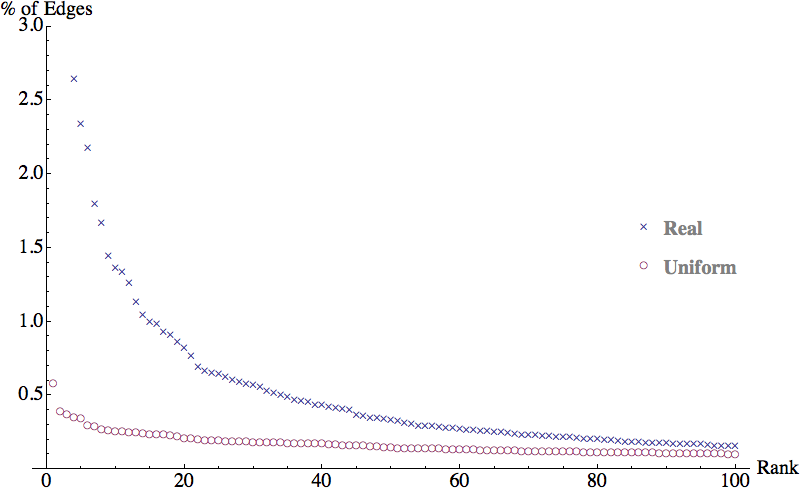
\includegraphics[width=0.5\textwidth]{images/cartesian_histogram.png}
\begin{minipage}{1\textwidth}
\caption{Histogram of percent edges between pairs of clusters. The long tail is omitted.}
\label{fig:cart-emp}
\vspace{-0.2in}
\end{minipage}
\end{figure}

\subsection{Hierarchical Tree Model}
\label{hierarchy}

%We assume that we are given a bipartite graph $G=(L,R,E)$.
In this model, the vertex sets $L$
and $R$ are the leaf sets of two full binary trees $T_L$ and $T_R$ of
depth $D$ where there is a one-to-one correspondence between the
subtrees of these two trees. We also assume that each branching in
both $T_L$ and $T_R$ splits the nodes evenly into the two
subtrees. As in the previous sections, we set $|L|/|R|=k$,
and require that this ratio is still $k$ if we divide the size of any subtree on the left
and that of its corresponding subtree on the right. For simplicity of notation, we
will use a subtree and its leaf set interchangeably. We assume that the trees are
fixed in advance but the bipartite recommendation graph $G = (L, R, E)$ is generated probabilistically according to
the following procedure. Let $u\in L$ and $T_L^0, \ldots T^{D-1}_L$ be
the subtrees it belongs at depths $0,\ldots, D-1$. Also, let
$T_R^0,\ldots, T_R^{D-1}$ be the subtrees on the right that correspond
to these trees on the left. We let $u$ make a recommending edge to $d_{D-1}$ of
the vertices in $T_{R}^{D-1}$, $d_{D-2}$ edges to the vertices in
$T_{R}^{D-2} \backslash T_{R}^{D-1}$ and so on. The $d_i$ edges out of $u$ are chosen uniformly from $T_R^i \setminus T_R^{i+1}$.
Let $d = d_{0} + \ldots + d_{D-1}$.\vs

\begin{figure}[b]
\vspace{-0.2in}
\centering
\begin{minipage}{0.45\textwidth}
\centering
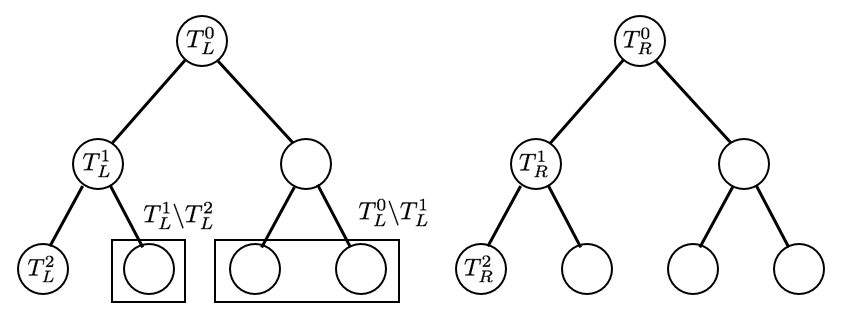
\includegraphics[width=1.1\textwidth]{images/hierarchy_tree.png}
%\begin{minipage}[h]{0.7\textwidth}
\caption{This diagram shows the notation we use for this model and the 1-to-1 correspondence of subtrees.}\label{fig:hierarchy}
\end{minipage}
\hspace{0cm}
\begin{minipage}{0.45\textwidth}
\centering
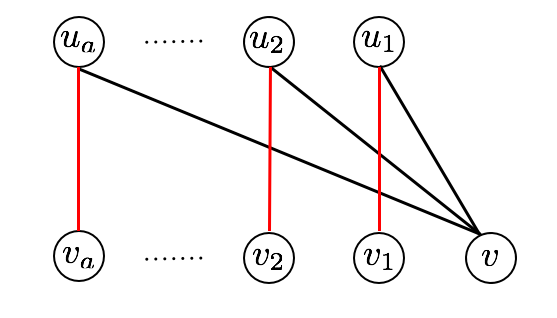
\includegraphics[width=0.9\textwidth]{images/greedy.png}

%\begin{minipage}[h]{.8\linewidth}

\vspace{-0.3in}
\caption{When $v$ selects edges to $u_1,\ldots, u_a$, it can remove $v_1,\ldots, v_a$ from candidates. Potentially invalidated edges shown in red.}

%\end{minipage}
\label{fig:greedy}
\end{minipage}
\end{figure}

For the $a=1$ case, our goal now is to find a $b$-matching~\cite{Gabow1983} in this
graph that is close to optimal in expectation. That is, our degree
upper and lower bounds on vertices in $L$ and $R$ are $c$ and 1
respectively. Let $c = c_0 + \ldots + c_{D-1}$ be similar to how we
defined $d$.  To combine the analysis of the randomness of the
algorithm and the randomness of the graph, the algorithm will pick
$c_{i}$ edges uniformly from among the $d_{i}$ edges going to each
level of the subtree to form a $(c,1)$-recommendation subgraph $H$.
This enables us to think of $H$ as being generated by the same process that generated $G$
but with fewer neighbors selected. With this model and
parameters in place, we can have the following analog of our main
theorem for $a=1$ for the hierarchical model and is proved in Appendix~\ref{sec:appendix}.

\begin{thm}
Let $S$ be the subset of edges $v\in R$ such that $\deg_H(v) \geq 1$ in the hierarchical tree model. Then
\[ \emph{\E}[S] \geq r(1-\exp(-ck)) \]
\end{thm}

%\begin{proof}
%Let $v\in R$ and let $T_L^{D-1}, T_L^{D-2}\backslash T_L^{D-1},
%\ldots, T_L^0\backslash T_L^1$ be the sets it can take edges
%from. Since $T_L$ and $T_R$ split perfectly evenly at each node the
%vertices in these sets will be chosen from $r_{D-1}, r_{D-1},
%r_{D-2},\ldots, r_{1}$ vertices in $R$ as neighbors,
%where $r_i$ is the size of subtree of the right tree rooted at depth
%$i$. Furthermore, each of these sets described above have size
%$l_{D-1}, l_{D-1}, l_{D-2}, \ldots, l_{1}$ respectively, where $l_i$
%is the size of a subtree of $T_L$ rooted at depth $i$. It follows that
%the probability that $v$ does not receive any edges at all is at most
%
%\begin{align*}
%	      \Pr[\lnot X_v]
%	&=    \left(1-\frac{1}{r_{D-1}}\right)^{c_0l_{D-1}}\prod_{i=1}^{D-1}\left(1 - \frac{1}{r_i}\right)^{c_{D-i} l_i} \\
%	&\leq \exp\left(-\frac{l_{D-1}}{r_{D-1}}c_0\right)\prod_{i=1}^{D-1} \exp\left(-\frac{l_i}{r_i}c_{D-i}\right) \\
%	&=    \exp\left(-(c_0 + \ldots + c_{D-1})k\right) \\
%	&=    \exp(-ck)
%\end{align*}
%
%Since this is an indicator variable, it follows that
%\[ \E[S] = \E\left[\sum_{v \in R} X_v \right] \geq r \left(1-\exp(-ck)\right) \]
%\end{proof}

Note that this is the same result as we obtained for the fixed degree
model in Section \ref{fixed-degree}. In fact, the approximation
guarantees when $ck \ll 1$ or $ck \gg 1$ hold exactly as before.\vs

The algorithmic sampling of $H$ is convenient in this model because we separated
out the edge generation process at a given depth from the edge
generation process at deeper subtrees.
%There is no ambiguity as to why
%an edge is in the underlying graph. That is,
If we superimpose $T_L$
and $T_R$, then an edge between $u\in L$ and $v\in R$ must have
come from an edge generated by the process corresponding to the lowest common ancestor of $u$ and $v$ in the same hierarchy. This way, the algorithm can actually sample intelligently and in the same way that the graph was generated in the first place, which is also the key to our simple analysis. Note
that we do not have to assume that the trees $T_L$ and $T_R$ are
binary. We only need the trees to be regular and evenly divided at
each vertex since the proof only relies on the proportions of the
sizes of the subtrees in $T_L$ and $T_R$.


\subsection{Cartesian Product Model}
\label{cartesian}
In this model, we assume that
$L$ has been partitioned into $t$ subsets $L_1,\ldots, L_t$ and
that $R$ has been partitioned into $t'$ subsets $R_1,\ldots,
R_{t'}$. For convenience, we let $|L_i| = l_i$ and $|R_j|=r_j$. Given
this, for each $1\leq i\leq t$ and each $1\leq j\leq t'$,
we let $G[L_i, R_j]$ be an instance of the fixed degree model with
$d=d_{ij}$. This allows us to assume different densities of edges between different pairs of clusters.
However, we require that for all $i$, we have $\sum_{j=1}^{t'}
d_{ij} = d$ for some fixed $d$. We also require that we have fixed in
advance $c_{ij} \leq d_{ij}$ for each $1\leq i\leq t$ and $1\leq j\leq t'$ that
satisfy $\sum_{j=1}^{t'} c_{ij} = c$ for all $i$ for some fixed $c$.
To sample $H$ from $G$, we sample $c_{ij}$ neighbors from $R_j$ for each
$u\in L_i$. Letting $S$ be the set of vertices in
$v\in R$ that satisfy $\deg_H(v)\geq 1$, we can show the following theorem
that is proved in Appendix~\ref{sec:appendix}.

\begin{thm}
Let $S$ be the subset of edges $v\in R$ such that $\deg_H(v) \geq 1$ in the cartesian product model. Then
%\vspace{-0.1in}
\[ \emph{\E}[S] \geq r - \sum_{j=1}^{t'} r_j \exp\left(-\sum_{i=1}^t c_{ij} \frac{l_i}{r_j}\right)\]
\end{thm}
%\begin{proof}
%Let $v_j \in R_j$ be an arbitrary vertex and let $X_{v_j}$ be the
%indicator variable for the event that $\deg_H(v_i) \geq 1$. The
%probability that none of the neighbors of some $u_i\in R_i$ is $v_j$
%is exactly $(1-\frac{1}{r_j})^{c_{ij}}$. It follows that the
%probability that the degree of $v_j$ in the subgraph $H[L_i,R_j]$ is 0
%is at most $(1-\frac{1}{r_j})^{c_{ij}l_i}$. Considering this
%probability over all $R_j$ gives us:
%\[ \Pr[X_{v_i} = 0] = \prod_{i=1}^{t} \left(1-\frac{1}{r_j}\right)^{c_{ij} l_i} \leq \exp\left(-\sum_{i=1}^t c_{ij} \frac{l_i}{r_j}\right)\]
%
%By linearity of expectation $\E[S] = \sum_{i=1}^{t'} r_i \E[X_{v_i}]$,
%so it follows that
%\[ \E[S] \geq \sum_{j=1}^{t'} r_j \left(1-\exp\left(-\sum_{i=1}^t c_{ij} \frac{l_i}{r_j}\right)\right) = r - \sum_{j=1}^{t'} r_j \exp\left(-\sum_{i=1}^t c_{ij} \frac{l_i}{r_j}\right)\]
%\end{proof}

%This model is interesting because it can capture a broader set of
%recommendation subgraphs than the fixed degree model. However, it is
%difficult to estimate how good a solution will be without knowing
%the sizes of the sets in the partitions. We note that we
%obtain the approximation guarantee of $(1-\exp(-ck))$ provided that
%$l_i/r_j = k$ for all $i$ and $j$ where $k$ is some fixed
%constant.
An powerful aspect of this model and the algorithm
we described for sampling $H$ is that we are free to select $c_{ij}$.
In particular, $c_{ij}$ can be chosen to maximize the
approximation guarantee in expectation we obtained above using
gradient descent or other first order methods prior to running the
recommendation algorithm to increases the quality of the solution.

\subsection{Weighted Model}
\label{weighted}
In all the models we have used so far we have assumed recommendation edges
all have the same weight. However, this assumption can be unrealistic in real life,
as recommendations from higher traffic pages might prove more valuable than those
with lower traffic. Furthermore, the similarity between pages and products can
also affect the effectiveness of a recommendation.

This motivates fixing the graph to be the
complete bipartite graph $K_{l,r}$, and giving the edges i.i.d weights
with mean $\mu$. We modify the objective function accordingly, so that
we count only the vertices in $R$ which have weight $\geq 1$. We now sample a recommendation subgraph
$H$ by simply sampling $c$ edges for each $u\in L$. If we
assume that $ck\mu \geq 1+\epsilon$ for some $\epsilon > 0$, then
this sampling solution still performs exceptionally well. If we let $S$ be the size of the
solution produced by this algorithm, we obtain the following theorem that is
proved in Appendix~\ref{sec:appendix}.

\begin{thm}
Let $G=K_{l,r}$ be a complete bipartite graph where the edges have i.i.d. weights and come from a distribution with mean $\mu$ that is supported on $[0,b]$; Assume that $ck\mu \geq 1+\epsilon$ for some $\epsilon > 0$. If the algorithm from Section \ref{fixed-degree} is used to sample a subgraph $H$ from $G$ and $S$ is the set of vertices in $R$ of incident weight at least one, then
\[ \emph{\E}[S] = \sum_{v\in R} \emph{\E}[X_v] = r\left(1-\exp\left(-\frac{2l\epsilon^2}{b^2}\right)\right) \]
\end{thm}
Since in real-life scenarios, $l >> (\frac{b}{\epsilon})^2$, the bound proved above is very close to optimal. Furthermore, as remarked in the Appendix, using negative correlation of the indicator variables of weight one in $R$, the result can also be turned into a high probability bound.

\iffalse
There are two things to note about this graph model. The first is that
since the variables $X_v$ are negatively correlated, our results in
Subsection \ref{fixed-degree} can be extended to the results of this
section. The second is that the condition that $W_{uv}$ are i.i.d
is not necessary to obtain the full effect of the analysis. Indeed,
the only place in the proof where the fact that $W_{uv}$ are i.i.d
is where we argue that $X_{uv}$ is large with high probability by a
Hoeffding bound. For the bound to apply, it is sufficient to assume
that $W_{uv}$ for all $v$ are independent. In particular, it is
possible that $W_{uv}$ for all $u$ are inter-dependent. This allows
us to assume a weight distribution that depends on the strength of
the recommender and the relevance of the recommendation separately.
\fi 
